% !TEX root = main.tex
\section{Quantifiers}
\begin{mytitle}[Approaches] We can either focus on model finding for which both an eager and a lazy approach exist. Or we can use E-matching, which does not generate models, but is good for $unsat$ results which are important for program verification. 
\end{mytitle}
\subsection{Definitions for Quantifiers}
\begin{mytitle}[Quantified Literal] A quantified literal is a formula $\forall x: T\ A$ or its negation $\lnot \forall x: T\ A$. Remember that $\exists x: T\ \lnot A \equiv \lnot\forall x: T\ A$.
\end{mytitle}
\begin{mytitle}[Ground term] A ground term is a term containing no (quantified) variables.
\end{mytitle}
\begin{mytitle}[Equalities]\hfill
\begin{itemize}
    \item $\forall x_1 \forall x_2 A \equiv \forall x_2 \forall x_1 A$
    \item $\exists x_1 \exists x_2 A \equiv \exists x_2 \exists x_1 A$
    \item $\lnot \forall x A \equiv \exists x \lnot A$ and $\lnot \exists x A \equiv \forall x \lnot A$
    \item $\forall x (A \land B) \equiv (\forall x A) \land (\forall x B)$
    \item $\exists x (A\lor B) \equiv (\exists x A) \lor (\exists x B)$
    \item If $x\not\in FV(A)$ then $\exists x A \equiv A \equiv \forall x A$ and $\forall x (A\lor B) \equiv A \lor (\forall x B)$ and $\exists x (A\land B) \equiv A \land (\exists x B)$ where $FV(A)$ are the free variables in $A$
\end{itemize}
\end{mytitle}

\subsection{Eager Approach}
\begin{mytitle}[Skolemization] Existential quantifiers in positive positions can be eliminated by replacing $\exists x A$ with $A[c/x]$ where $c$ is a fresh constant. In general, Skolemization replaces an $\exists$-bound variable with a fresh function of the $\forall$-bound variables enclosing it. For example $\forall x: Int\ \exists y: Int\ (y > x)$ becomes $\forall x: Int\ (f(x) > x)$.
\end{mytitle}
\begin{mytitle}[Eager Quantifier Elimination] We can allow only formulas of the form $\exists x_1\ldots \exists x_m$ $\forall y_1 \ldots \forall y_n A$ where $A$ is quantifier free and we have no function symbols except constants and equality. Then we can apply Skolemization to remove the $\exists$ quantifiers. After that it is sufficient to instantiate the $\forall$ quantifiers for each constant. For example $\forall x: T\ A$ becomes $A[c_1/x]\land A[c_2/x]\land \ldots$. The result is equi-satisfiable and quantifier-free.
\end{mytitle}

\subsection{Lazy Approach}
\begin{mytitle}[Extended clause] An extended clause is a disjunction of first-order literals and quantified literals.
\end{mytitle}
\begin{mytitle}[Extended CNF] A formula is in extended CNF iff it is a conjunction of extended clauses. Two examples:
\begin{itemize}
    \item $(\forall x:T\ p(x))\To \forall y:T\ q(y)$ has extended CNF form $(\lnot \forall x:T\ p(x))\lor\forall y:T\ q(y)$
    \item $(\exists x:T\ \lnot p(x)) \lor \forall y:T\ q(y)$ has extended CNF form $\lnot p(c)\lor \forall y:T\ q(y)$
\end{itemize}
\end{mytitle}
\begin{mytitle}[Lazy Quantifier Elimination] We extend propositional abstraction to also abstract quantified literals. For example $\lnot p(c) \lor \forall y:T\ q(y)$ becomes $\lnot a \lor b$. We do not cover more details in this lecture.
\end{mytitle}

\subsection{E-Matching}
\begin{mytitle}[E-graph] We use this graph to represent equalities and disequalities. We have a node labelled $f$ for each ground term $f(\ldots)$. We have directed, indexed edges to each function argument. We express equality with a green double line and disequality with a red single line. When adding an $a$ to $b$ equality edge, we need to find the pairs of nodes for each function $f$. If the arguments on the two $f$ nodes are pairwise equal, we equate them too. This is an efficient way to track (dis)equalities and yields a theory solver for $T_E$.
\end{mytitle}
\begin{center}
\begin{minipage}{0.49\textwidth}
\begin{center}
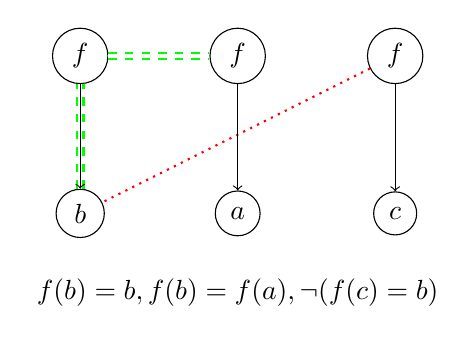
\begin{tikzpicture}
\node (b) [draw, circle, minimum size=0.8, align=center] at (0,0) {$b$};
\node (a) [draw, circle, minimum size=0.8, align=center] at (2,0) {$a$};
\node (c) [draw, circle, minimum size=0.8, align=center] at (4,0) {$c$};
\node (f1) [draw, circle, minimum size=0.8, align=center] at (0,2) {$f$};
\node (f2) [draw, circle, minimum size=0.8, align=center] at (2,2) {$f$};
\node (f3) [draw, circle, minimum size=0.8, align=center] at (4,2) {$f$};

\draw [double, dashed, thick, green, double distance=1.5] (b) -- (f1);
\draw [double, dashed, thick, green, double distance=1.5] (f1) -- (f2);
\draw [red, dotted, thick] (f3) -- (b);
\draw [->] (f1) -- (b);
\draw [->] (f2) -- (a);
\draw [->] (f3) -- (c);

\node [align=center] at (2, -1) {$f(b) = b, f(b)=f(a), \lnot(f(c)=b)$};
\end{tikzpicture}
\end{center}
\end{minipage}
\begin{minipage}{0.49\textwidth}
\begin{center}
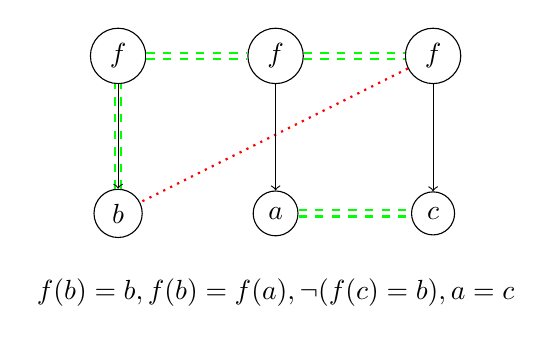
\begin{tikzpicture}
\node (b) [draw, circle, minimum size=0.8, align=center] at (0,0) {$b$};
\node (a) [draw, circle, minimum size=0.8, align=center] at (2,0) {$a$};
\node (c) [draw, circle, minimum size=0.8, align=center] at (4,0) {$c$};
\node (f1) [draw, circle, minimum size=0.8, align=center] at (0,2) {$f$};
\node (f2) [draw, circle, minimum size=0.8, align=center] at (2,2) {$f$};
\node (f3) [draw, circle, minimum size=0.8, align=center] at (4,2) {$f$};

\draw [double, dashed, thick, green, double distance=1.5] (b) -- (f1);
\draw [double, dashed, thick, green, double distance=1.5] (f1) -- (f2);
\draw [double, dashed, thick, green, double distance=1.5] (a) -- (c);
\draw [double, dashed, thick, green, double distance=1.5] (f2) -- (f3);
\draw [red, dotted, thick] (f3) -- (b);
\draw [->] (f1) -- (b);
\draw [->] (f2) -- (a);
\draw [->] (f3) -- (c);

\node [align=center] at (2, -1) {$f(b) = b, f(b)=f(a), \lnot(f(c)=b), a=c$};
\end{tikzpicture}
\end{center}
\end{minipage}
\captionof{figure}{Example E-graphs}
\end{center}

\begin{mytitle}[Extended quantifier syntax] We add two extensions to $\forall$-quantified formulas:
    \begin{mysubtitle}[Merging quantifiers] We allow multiple adjacent $\forall$-quantifiers to be merged into one. For example $\forall x_1 \forall x_2 A$ becomes $\forall x_1, x_2 A$.
    \end{mysubtitle}
    \begin{mysubtitle}[Triggers] We allow a trigger to be attached to any $\forall$-quantifier. For example $\forall x \{t\} A$. This term $t$ is of any sort and satisfies the following: $t$ must contain all the variables quantified by the quantifier, $t$ may not contain interpreted function symbols except for constants and $t$ must contain at least one non-constant function symbol. For example $\forall x: Int\ \{f(x)\} f(x) < b$.
    \end{mysubtitle}
\end{mytitle}
\begin{mytitle}[Matching a trigger] A quantifier $\forall x. \{t\}\ A$ will only be instantiated when there is a ground term $t[t'/x]$ in the current formula. In this case $A[t'/x]$ is conjoined to the current formula. For example in the formula $g(f(a))=0 \land \forall x: Int\ \{g(f(x))\} g(f(x)) = 1$ the term $g(f(a))$ matches the trigger $g(f(x))$ (with $t'=a$), causing the instantiation $g(f(a))=1$.
\end{mytitle}
\begin{mytitle}[E-matching] A quantifier $\forall x\{t\} A$ will only be instantiated when there are ground terms $t'$ and $t''$ such that $t''$ occurs in our current formula to satisfy / our current model and $t[t'/x] = t''$ is true in our current model. Triggers are matched modulo equalities. E-matching can be efficiently implemented by pattern-matching triggers against the current E-graph.
\end{mytitle}
\begin{center}
\begin{minipage}{0.49\textwidth}
\begin{center}
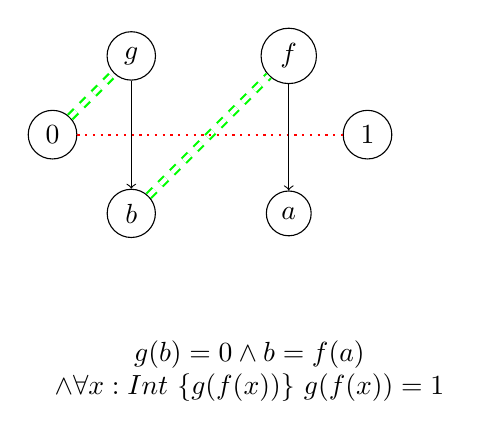
\begin{tikzpicture}
\node (b) [draw, circle, minimum size=0.8, align=center] at (0,0) {$b$};
\node (a) [draw, circle, minimum size=0.8, align=center] at (2,0) {$a$};
\node (g) [draw, circle, minimum size=0.8, align=center] at (0,2) {$g$};
\node (f) [draw, circle, minimum size=0.8, align=center] at (2,2) {$f$};
\node (0) [draw, circle, minimum size=0.8, align=center] at (-1,1) {$0$};
\node (1) [draw, circle, minimum size=0.8, align=center] at (3,1) {$1$};

\draw [double, dashed, thick, green, double distance=1.5] (0) -- (g);
\draw [double, dashed, thick, green, double distance=1.5] (b) -- (f);
\draw [red, dotted, thick] (0) -- (1);

\draw [->] (g) -- (b);
\draw [->] (f) -- (a);

\node [align=center] at (1.5,-2) {$g(b)=0 \land b=f(a)$\\ $\land \forall x:Int\ \{g(f(x))\}\ g(f(x))=1$};
\end{tikzpicture}
\end{center}
\end{minipage}
\begin{minipage}{0.49\textwidth}
\begin{center}
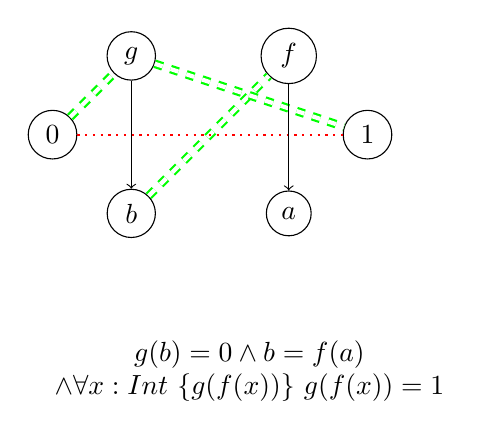
\begin{tikzpicture}
\node (b) [draw, circle, minimum size=0.8, align=center] at (0,0) {$b$};
\node (a) [draw, circle, minimum size=0.8, align=center] at (2,0) {$a$};
\node (g) [draw, circle, minimum size=0.8, align=center] at (0,2) {$g$};
\node (f) [draw, circle, minimum size=0.8, align=center] at (2,2) {$f$};
\node (0) [draw, circle, minimum size=0.8, align=center] at (-1,1) {$0$};
\node (1) [draw, circle, minimum size=0.8, align=center] at (3,1) {$1$};

\draw [double, dashed, thick, green, double distance=1.5] (0) -- (g);
\draw [double, dashed, thick, green, double distance=1.5] (b) -- (f);
\draw [double, dashed, thick, green, double distance=1.5] (g) -- (1);
\draw [red, dotted, thick] (0) -- (1);

\draw [->] (g) -- (b);
\draw [->] (f) -- (a);

\node [align=center] at (1.5,-2) {$g(b)=0 \land b=f(a)$\\ $\land \forall x:Int\ \{g(f(x))\}\ g(f(x))=1$};
\end{tikzpicture}
\end{center}
\end{minipage}
\captionof{figure}{E-graph before and after E-matching}
\end{center}
\begin{mytitle}[Integrating E-matching] \hfill
\begin{enumerate}
    \item Run a DPLL-like search on the propositional abstraction $A^P$ of the input formula $A$.
    \item Maintain the current (dis)equality information in an E-graph.
    \item When a quantified literal is added to the candidate model, record the quantifier for potential E-matching later.
    \item Periodically, run an E-matching engine on the current E-graph. Look for new instantiations of recorded quantifiers and add them. This expands the current formula for the DPLL search. This procedure will only return $unsat$ or $unknown$, no model.
\end{enumerate}
\end{mytitle}
\begin{mytitle}[Selecting triggers] Triggers may be too restrictive, leading to missed relevant instances or too permissive, leading to too many instantiations. Triggers may in general consist of sets of terms, either $\{f(x), g(x)\}$, where it will only be instantiated when we have both $f(t)$ and $g(t)$ for some $t$ or $\{f(x)\}\{g(x)\}$ where it will be instantiated if we have either $f(t)$ or $g(t)$ for some $t$.
\end{mytitle}
\begin{mytitle}[Matching Loop] A situation that leads to infinite instantiations is called a matching loop.
\end{mytitle}